% =====================================================================
% Documento da Etapa 1 --- Modelagem e Planejamento da Solução
% Template oficial da SBC (sbc-template.sty e sbc.bst estão nesta pasta).
% Cada pessoa edita SÓ a própria seção em secoes/ (veja o README.md).
% Compilar: pdflatex etapa1 && bibtex etapa1 && pdflatex etapa1 && pdflatex etapa1
% Antes de entregar, não pode sobrar nenhum \pendente{...} (aparece em vermelho no PDF).
% =====================================================================
\documentclass[12pt]{article}

\usepackage{sbc-template}
\usepackage{graphicx,url}
\usepackage[utf8]{inputenc}
\usepackage[T1]{fontenc}
\usepackage[brazil]{babel}
\usepackage{amsmath}
\usepackage{booktabs,tabularx,array}
\usepackage{xcolor}

\newcolumntype{Y}{>{\raggedright\arraybackslash}X}
\graphicspath{{figuras/}}

% Código e nomes de função: \codigo{bfs}
\newcommand{\codigo}[1]{\texttt{#1}}
% Lembrete em vermelho; nenhum pode sobrar na versão entregue.
\newcommand{\pendente}[1]{\textcolor{red}{[PENDENTE: #1]}}

\sloppy

\title{Identificação de influenciadores na rede da Twitch em português:\\
       modelagem e planejamento (Etapa 1)}

% Completar os nomes completos de todos (como no Canvas) e trocar os Sobrenome em vermelho.
\author{Brunno Enrico Machado Costa\inst{1}, Vitória Rani Santos Menezes\inst{1}, Kaio Ferreira\inst{1},\\
  Iago \textcolor{red}{Sobrenome}\inst{1}, Arthur \textcolor{red}{Sobrenome}\inst{1}, Ravi \textcolor{red}{Sobrenome}\inst{1}}

\address{\pendente{curso, disciplina e instituição}}

\begin{document}

\maketitle

\begin{resumo}
  Este documento apresenta a modelagem e o planejamento de uma ferramenta, escrita em
  Python puro, que analisa redes sociais com grafos. O problema aplicado é identificar os
  influenciadores da rede de streamers da Twitch em português (1.912 nós e 31.299 arestas)
  e verificar qual medida de centralidade os encontra melhor, comparando cada ranking com o
  alcance numa simulação de espalhamento SIR e com as visualizações reais dos canais.
  Descrevemos o problema, as quatro bases de dados, a modelagem do grafo em lista de
  adjacência, os diagramas UML e o plano de desenvolvimento até a entrega final.
\end{resumo}

% =====================================================================
% Descrição formal do problema aplicado --- Ravi (Frente 5)
% Só o Ravi edita este arquivo. Apague os \pendente ao escrever.
% =====================================================================
\section{Problema aplicado}\label{sec:problema}

\pendente{Ravi: descrição formal do problema, com quatro partes.}

\paragraph{Pergunta.} \pendente{Quais streamers são os influenciadores da rede da Twitch em
português, e qual medida de centralidade os encontra melhor? Citar a pergunta de
\cite{kitsak2010}: o k-core prevê os espalhadores melhor que o grau?}

\paragraph{Entrada.} \pendente{O grafo da Twitch PT (Seção~\ref{sec:bases}) e os atributos de cada
streamer (visualizações, parceiro).}

\paragraph{Saída.} \pendente{Um ranking dos streamers para cada centralidade (grau, proximidade,
harmônica, intermediação, PageRank e k-core) e o $\tau$ de Kendall de cada ranking contra a
referência.}

\paragraph{Como validar.} \pendente{Simulação SIR a partir de cada nó (alcance médio), com $\beta$
um pouco acima do limiar epidêmico (0,0079); comparação de cada ranking com o alcance e com as
visualizações reais pelo $\tau$ de Kendall~\cite{kendall1938}.}
       % Ravi
% =====================================================================
% Bases de dados --- Brunno (Frente 1)
% =====================================================================
\section{Bases de dados}\label{sec:bases}

Usamos quatro redes públicas e já anonimizadas, baixadas das fontes originais. Por serem
arquivos fixos, os experimentos podem ser repetidos por qualquer pessoa. A Tabela~\ref{tab:bases}
resume as bases; os tamanhos foram conferidos pelos testes automáticos dos leitores
(\codigo{tests/test\_leitores.py}).

\begin{table}[htbp]
\centering
\caption{Bases de dados usadas no trabalho: $n$ nós, $m$ arestas e densidade $2m/(n(n-1))$.}
\label{tab:bases}
\small
\begin{tabularx}{\textwidth}{@{}>{\raggedright\arraybackslash}p{3.3cm} r r r Y@{}}
\toprule
Base & $n$ & $m$ & Densidade & Papel no trabalho \\
\midrule
Twitch PT & 1.912 & 31.299 & 0,0171 & Base principal: ranking de influenciadores \\
ego-Facebook & 4.039 & 88.234 & 0,0108 & Segunda rede real, maior: desempenho \\
Network of Thrones (livro 3) & 303 & 1.008 & 0,0220 & Demonstração (rede com peso) \\
Karate Club & 34 & 78 & 0,1390 & Testes de corretude (valores publicados) \\
\bottomrule
\end{tabularx}
\end{table}

\paragraph{Twitch PT.} Rede de amizades mútuas entre streamers que transmitem em português,
coletada por \cite{rozemberczki2021} e distribuída pelo SNAP~\cite{leskovec2014snap}. Cada nó
traz atributos reais: número de visualizações, se o canal é parceiro da Twitch (279 dos 1.912),
se tem conteúdo adulto e há quantos dias existe. As visualizações servem de validação externa
para o ranking de influenciadores.

\paragraph{ego-Facebook.} União de dez redes ego de amizades do Facebook, com os
identificadores anonimizados~\cite{mcauley2012}. É maior e mais densa em triângulos que a
Twitch PT, o que a torna boa para medir o desempenho dos algoritmos.

\paragraph{Network of Thrones.} Personagens do terceiro livro de \emph{As Crônicas de Gelo e
Fogo}; dois personagens se ligam quando os nomes aparecem a até 15 palavras um do outro, e o peso
é o número de vezes em que isso acontece~\cite{beveridge2016}. Usamos o arquivo do repositório
dos autores, com 303 personagens e 1.008 arestas (o artigo original cita uma versão menor).
Como o público reconhece os personagens, a rede é ótima para a demonstração.

\paragraph{Karate Club.} Clube de caratê estudado por \cite{zachary1977}, que se dividiu em
dois grupos (17 membros cada). Os valores conhecidos dessa rede, como o agrupamento médio de
0,5706 e a modularidade máxima de 0,4198, servem para provar que os algoritmos estão corretos.
          % Brunno
% =====================================================================
% Modelagem do grafo: justificativa e diagrama de classes --- Brunno (Frente 1)
% =====================================================================
\section{Modelagem do grafo}\label{sec:modelagem}

\subsection{O que é nó e o que é aresta}

Cada rede vira um grafo $G = (V, E)$ não direcionado e simples (sem arestas repetidas),
com $n = |V|$ nós e $m = |E|$ arestas. Na Twitch PT, cada nó é um streamer e cada aresta é
uma amizade mútua, sem peso. No ego-Facebook, os nós são usuários e as arestas, amizades.
No Karate Club, os nós são membros do clube e as arestas, interações fora das aulas. Na
Network of Thrones, os nós são personagens e cada aresta tem peso $w(e)$ igual ao número de
interações entre os dois no livro. Grafos sem peso usam $w(e) = 1$.

\subsection{Por que lista de adjacência}

As redes sociais são esparsas: cada pessoa se liga a uma fração pequena das outras. Na
Twitch PT, a densidade é $2m/(n(n-1)) \approx 0{,}017$, ou seja, só 1,7\% dos pares possíveis
são amizades. Uma matriz de adjacência guardaria $n^2 = 3{,}66$ milhões de células, 98\% delas
com zero, e gastaria $O(n^2)$ de memória. A lista de adjacência guarda só as arestas que
existem, em $O(n + m)$, e percorre os vizinhos de um nó $v$ em $O(\text{grau}(v))$. Por isso
a busca em largura custa $\Theta(n + m)$ com lista e $\Theta(n^2)$ com
matriz~\cite{cormen2022,sedgewick2011}, e quase todos os algoritmos do trabalho dependem
desse percurso.

\subsection{Por que um dicionário de dicionários}

A classe \codigo{Grafo} guarda a lista de adjacência como um dicionário de dicionários:
\codigo{\_adj[v][w]} é o peso da aresta entre $v$ e $w$. Três motivos levaram a essa escolha:
\begin{itemize}
  \item testar se uma aresta existe custa $O(1)$ em média, enquanto um dicionário de listas
        exigiria percorrer os vizinhos, em $O(\text{grau}(v))$~\cite{pythoncomplexidade};
  \item o peso fica junto do vizinho, o que atende a Network of Thrones e o Louvain, que cria
        arestas com peso ao agrupar comunidades~\cite{blondel2008};
  \item os nós podem ser de qualquer tipo imutável: números na Twitch e nomes na Network of Thrones.
\end{itemize}
O NetworkX, que só usaremos para comparar desempenho, adota a mesma estrutura pelos mesmos
motivos~\cite{hagberg2008}. A Tabela~\ref{tab:complexidade} resume o custo das operações.

\begin{table}[htbp]
\centering
\caption{Custo das operações da classe \codigo{Grafo} ($O(1)$ em média, pelo uso de dicionários).}
\label{tab:complexidade}
\small
\begin{tabular}{@{}l l@{}}
\toprule
Operação & Tempo \\
\midrule
Inserir nó, inserir ou remover aresta & $O(1)$ \\
Testar aresta, ler peso, grau & $O(1)$ \\
Percorrer os vizinhos de $v$ & $O(\text{grau}(v))$ \\
Listar todas as arestas & $O(n + m)$ \\
Número de nós e de arestas & $O(1)$ \\
Memória total & $O(n + m)$ \\
\bottomrule
\end{tabular}
\end{table}

\subsection{Outras decisões}

\begin{itemize}
  \item \textbf{Grafos direcionados:} a classe também os aceita. Nesse caso, guarda à parte os
        predecessores de cada nó (\codigo{\_pred}), para calcular o grau de entrada e o
        PageRank~\cite{brin1998} sem percorrer o grafo inteiro. No não direcionado,
        \codigo{\_pred} é o próprio \codigo{\_adj}, sem cópia.
  \item \textbf{Laços:} a classe aceita a aresta $(v, v)$, que o Louvain cria ao agrupar
        comunidades, e a conta duas vezes no grau, para a soma dos graus ser sempre $2m$.
        Os leitores das bases descartam laços, que nelas são ruído.
  \item \textbf{Contador de arestas:} o número de arestas $m$ é mantido a cada inserção e
        remoção, e sai em $O(1)$; ele aparece na densidade, no grau médio e na modularidade.
  \item \textbf{Reindexação:} nos algoritmos pesados (betweenness de Brandes e PageRank), os nós
        são renumerados de $0$ a $n-1$ e a adjacência vira uma lista de listas, que tem custo
        constante menor que o dicionário.
\end{itemize}

\subsection{Diagramas de classes e de pacotes}

A Figura~\ref{fig:classes} detalha o núcleo: a classe \codigo{Grafo} e o
\codigo{IndexadorDeNos}, que renumera os nós de $0$ a $n-1$ para os algoritmos pesados.
A Figura~\ref{fig:pacotes} mostra como o resto do código se organiza em volta dele. Os demais
pacotes são módulos de funções que recebem um \codigo{Grafo}, não o alteram e devolvem um
resultado por nó (\codigo{dict[nó, valor]}), um contrato comum a todas as frentes. Os leitores
e os geradores criam grafos; a interface só chama as funções e mostra os resultados. O NetworkX
aparece apenas em \codigo{desempenho/}, para a comparação permitida pelo enunciado.

\begin{figure}[htbp]
\centering
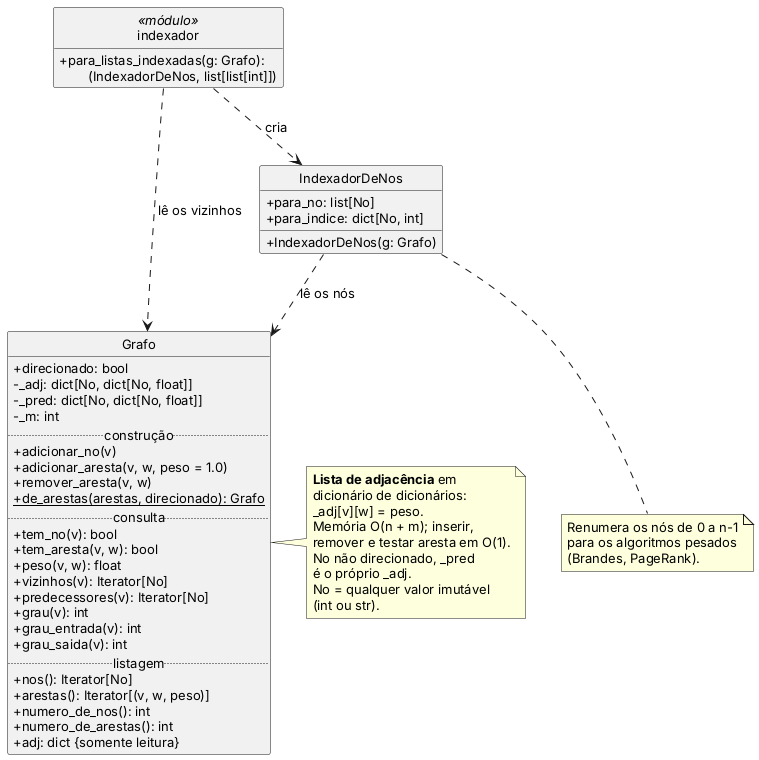
\includegraphics[width=.9\textwidth]{classes.png}
\caption{Diagrama de classes do núcleo (\codigo{redes/nucleo}).}
\label{fig:classes}
\end{figure}

\begin{figure}[htbp]
\centering
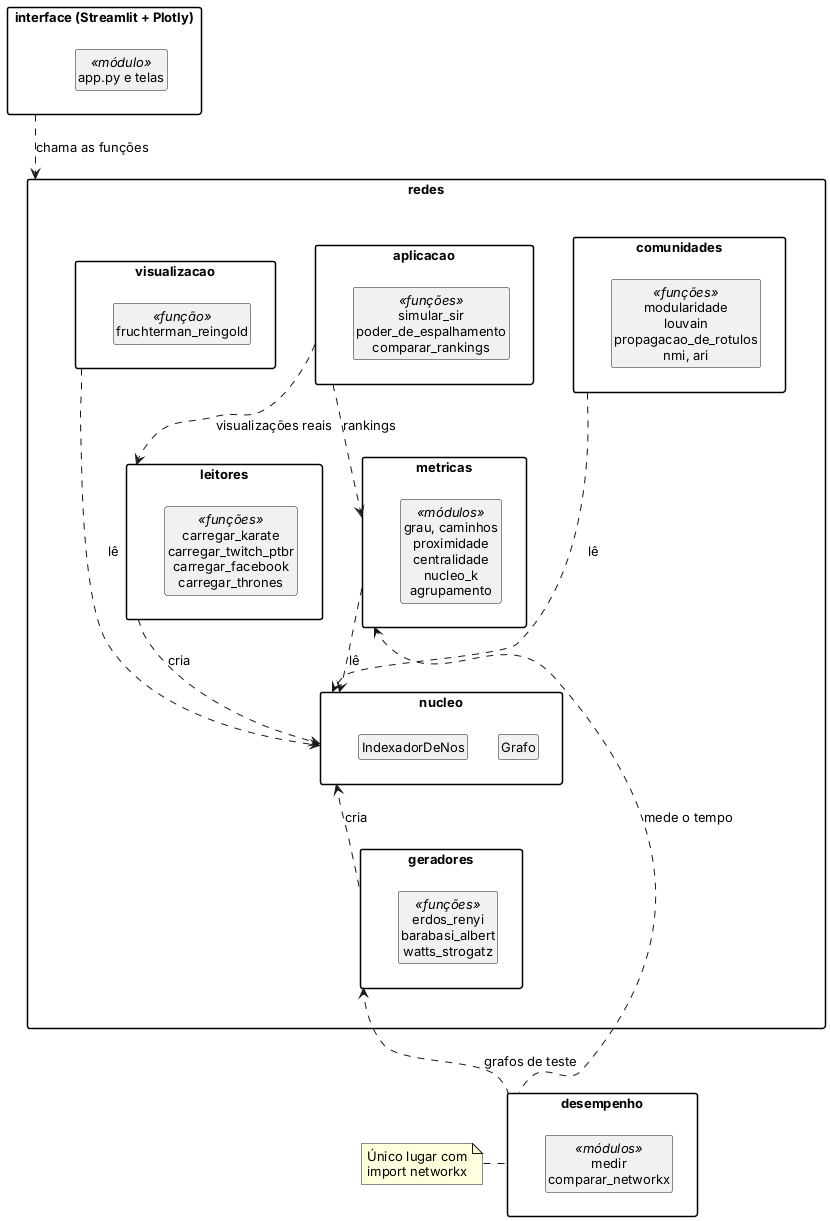
\includegraphics[width=.85\textwidth]{pacotes.png}
\caption{Diagrama de pacotes da ferramenta. As setas tracejadas indicam dependência: quem
  aponta usa o pacote apontado.}
\label{fig:pacotes}
\end{figure}
      % Brunno
% =====================================================================
% Diagrama de casos de uso e esboço das telas --- Kaio (Frente 6)
% Só o Kaio edita este arquivo. Texto inicial montado a partir de
% documentos/uml/casos_de_uso.md (PR #5); o Kaio revisa e completa.
% =====================================================================
\section{Casos de uso e telas}\label{sec:casos}

A Figura~\ref{fig:casos} mostra os casos de uso da ferramenta. Há dois atores: o
\emph{usuário (analista)}, que opera a interface, e as \emph{bases de dados}, um sistema externo
que a ferramenta só lê. Os 17 casos de uso cobrem obter um grafo (carregando uma base real ou
gerando um grafo sintético), calcular métricas, detectar comunidades, identificar
influenciadores com a simulação SIR, visualizar a rede e ver ou exportar os resultados. A
descrição de cada caso de uso, com pré-condições e fluxos, está em
\codigo{documentos/uml/casos\_de\_uso.md}.

\begin{figure}[htbp]
\centering
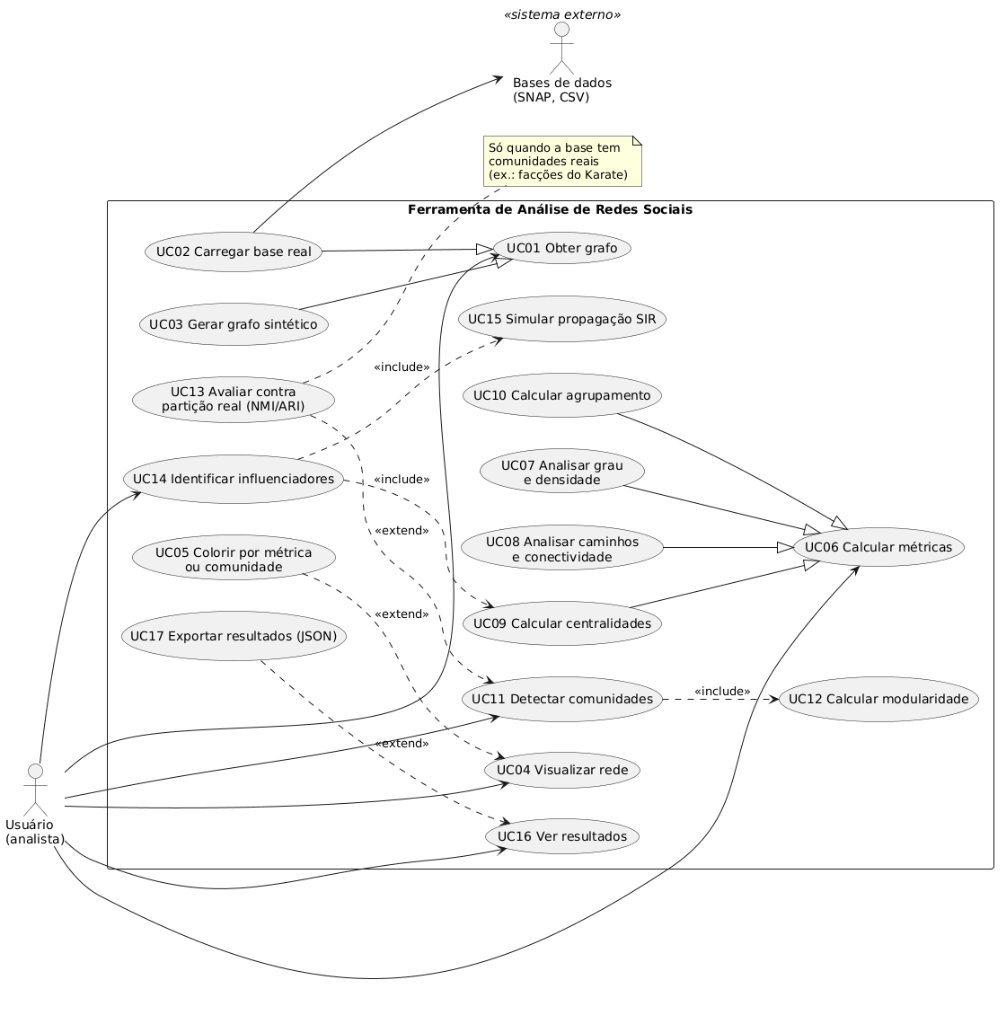
\includegraphics[width=.95\textwidth]{casos_de_uso.jpg}
\caption{Diagrama de casos de uso da ferramenta.}
\label{fig:casos}
\end{figure}

\pendente{Kaio: esboço das seis telas da interface (visão geral, rede, centralidades,
comunidades, influenciadores e desempenho).}
   % Kaio
% =====================================================================
% Diagrama de sequência --- Iago (Frente 3)
% Só o Iago edita este arquivo. Salve a imagem em figuras/ e o código-fonte
% (PlantUML) em documentos/uml/.
% =====================================================================
\section{Diagrama de sequência}\label{sec:sequencia}

A Figura~\ref{fig:sequencia} mostra as mensagens trocadas quando o usuário pede o ranking de
influenciadores da Twitch PT (caso de uso UC14, que inclui o UC09, calcular centralidades). O
fluxo passa por quatro camadas: usuário, interface, centralidades e grafo.

\begin{figure}[htbp]
\centering
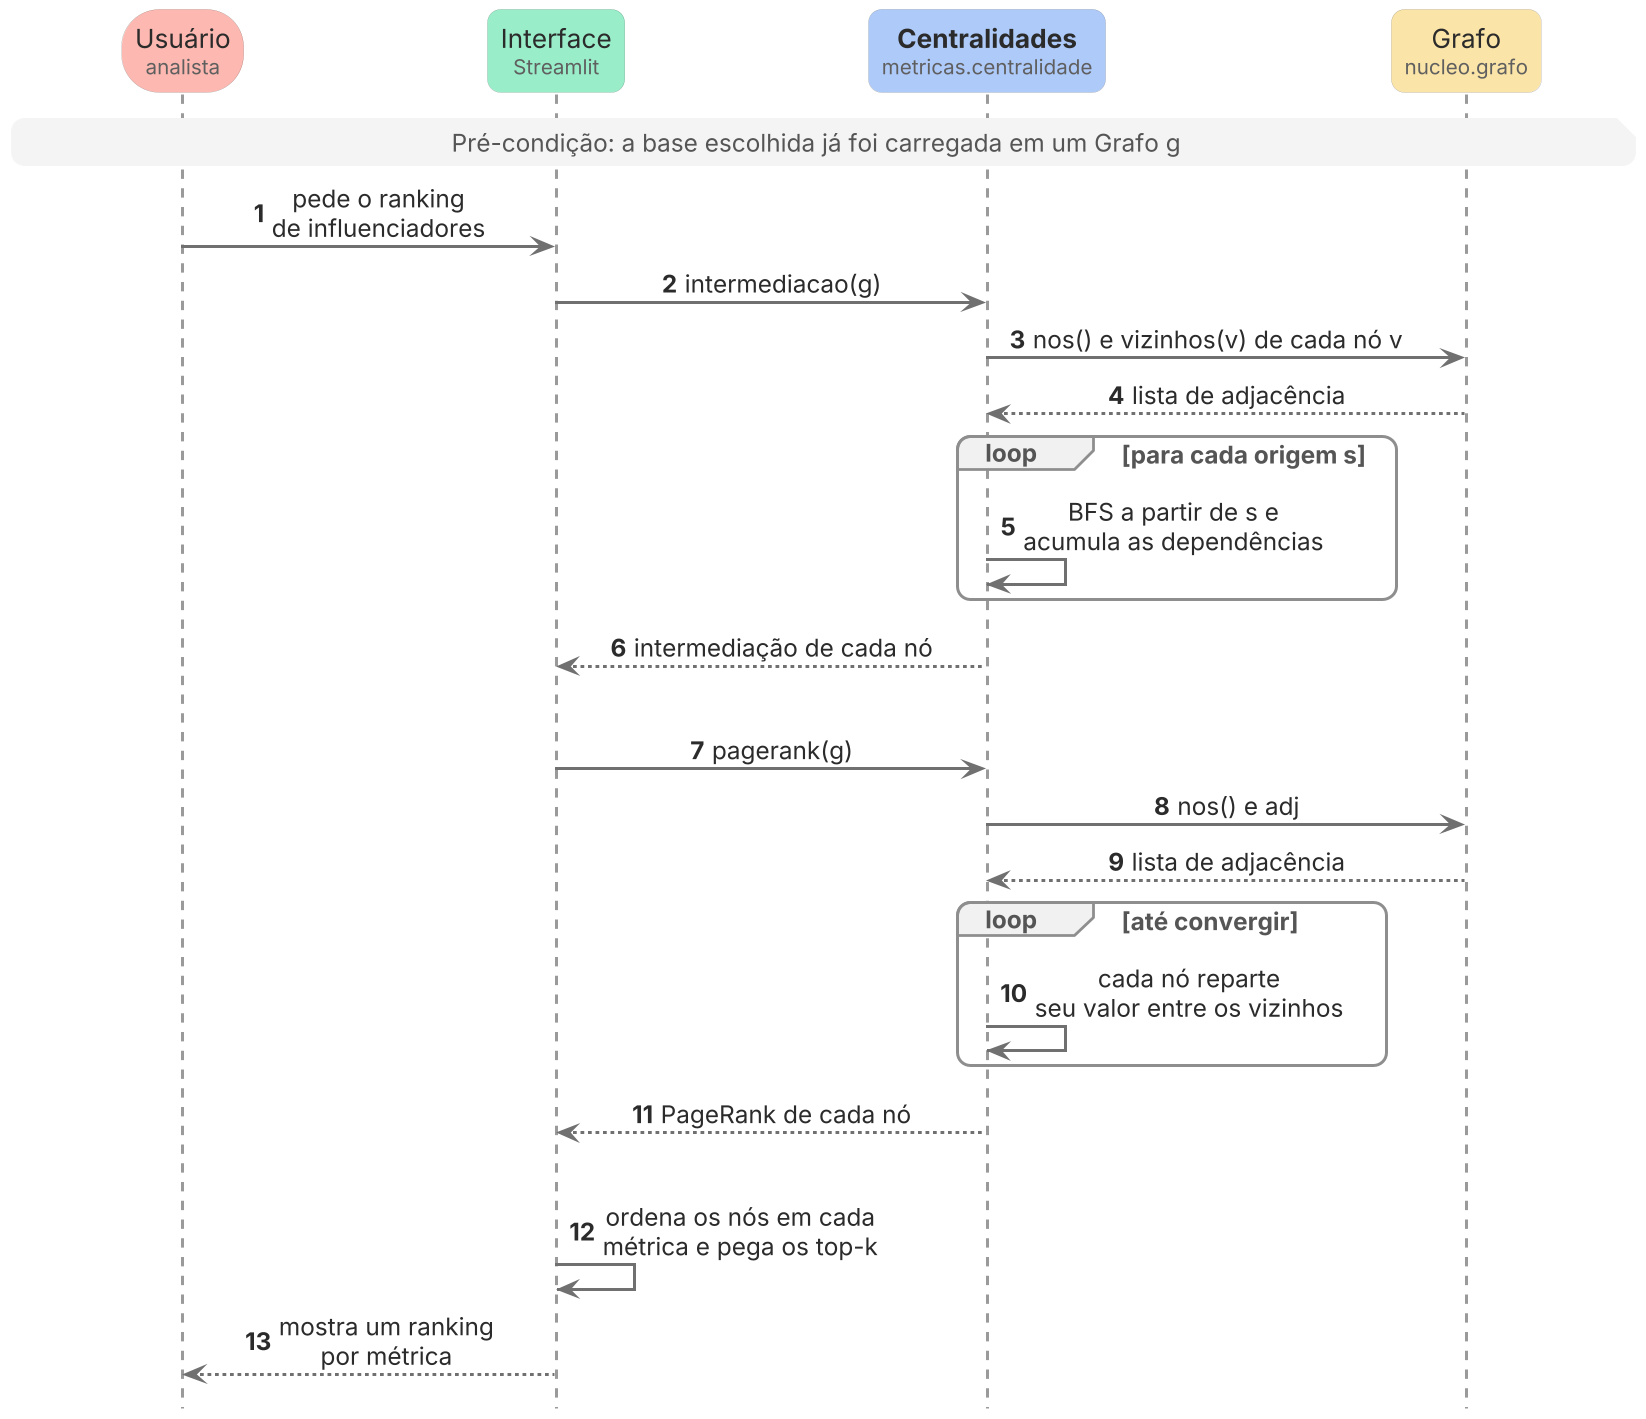
\includegraphics[width=\textwidth]{sequencia.png}
\caption{Diagrama de sequência do ranking de influenciadores.}
\label{fig:sequencia}
\end{figure}

O diagrama parte de um grafo já carregado. Quando o usuário pede o ranking (mensagem 1), a
interface chama \codigo{intermediacao(g)} (mensagem 2). A função lê os nós e os vizinhos do
grafo uma única vez, em $O(n + m)$, e monta uma lista de adjacência indexada por inteiros
(mensagens 3 e 4). Depois, o algoritmo de Brandes~\cite{brandes2001} faz uma busca em largura a
partir de cada origem $s$, conta os caminhos mínimos que saem de $s$ e acumula a parcela de
cada nó nesses caminhos (mensagem 5), sem voltar a consultar o grafo. Como são $n$ buscas de
custo $O(n + m)$, o total é $O(nm)$; na versão por amostragem, só $k$ origens sorteadas entram
no laço, em $O(km)$, e o resultado é multiplicado por $n/k$ para estimar o valor
exato~\cite{brandes2007}. A função devolve um valor por nó (mensagem 6). O
\codigo{pagerank(g)} segue o mesmo padrão: lê a adjacência uma vez (mensagens 8 e 9) e repete
a distribuição dos valores entre os vizinhos até convergir (mensagem 10). O k-core
(\codigo{numero\_de\_nucleo}), a terceira centralidade da Frente 3, segue o mesmo padrão (lê o
grafo uma vez e calcula sobre a lista indexada) e foi omitido para o diagrama não ficar longo.
Por fim, a interface ordena os nós em cada métrica, pega os $k$ primeiros e mostra um ranking por métrica
(mensagens 12 e 13). As métricas não são somadas: comparar os rankings entre si e com o alcance
na simulação SIR é o papel do módulo \codigo{aplicacao} (Seção~\ref{sec:problema}). As
centralidades só chamam métodos de consulta do \codigo{Grafo} e nunca o alteram, como exigem as
regras do grupo.
      % Iago
% =====================================================================
% Diagrama de atividades do Louvain --- Arthur (Frente 4)
% Só o Arthur edita este arquivo. Salve a imagem em figuras/ e o código-fonte
% (PlantUML) em documentos/uml/.
% =====================================================================
\section{Diagrama de atividades do Louvain}\label{sec:atividades}

O algoritmo de Louvain~\cite{blondel2008} é um método heurístico eficiente para detecção de
 comunidades em redes complexas por meio da maximização da modularidade ($Q$). 
 A Figura~\ref{fig:atividades} apresenta o diagrama de atividades do algoritmo, 
 que opera em duas fases interdependentes executadas iterativamente até a convergência global.

Na \textbf{Fase 1 (Otimização Local)}, cada vértice inicia em sua própria comunidade individual. 
Os nós são visitados em ordem pseudo-aleatória 
(determinada por uma semente fixa para garantir reprodutibilidade). 
Para cada nó $v$, avalia-se o ganho de modularidade ($\Delta Q$) resultante de sua remoção 
da comunidade atual e inserção na comunidade de cada um de seus vizinhos. 
Se houver ganho estritamente positivo ($\Delta Q > 0$), o nó é transferido para a 
comunidade que proporcionar o maior aumento; caso contrário, ele permanece em sua posição original. 
Esse processo é repetido sequencialmente sobre todos os vértices até que nenhum nó mude de comunidade, 
alcançando um ótimo local.

Na \textbf{Fase 2 (Agregação da Rede)}, constrói-se um novo grafo ponderado reduzido, 
no qual cada comunidade obtida na primeira fase é colapsada em um único supernó. 
As arestas internas entre membros da mesma comunidade convertem-se em laços (\emph{self-loops}) 
com pesos somados, enquanto as conexões entre comunidades distintas tornam-se arestas ponderadas 
entre os respectivos supernós. 

O laço externo repete a Fase 1 sobre o grafo agregado resultante. O algoritmo encerra 
sua execução quando a modularidade global da rede estabiliza ($\Delta Q \le 0$). 
Ao final, a estrutura hierárquica de supernós é desempacotada, retornando a partição mapeada para 
os identificadores originais dos vértices e a modularidade final alcançada.

\begin{figure}[htbp]
\centering
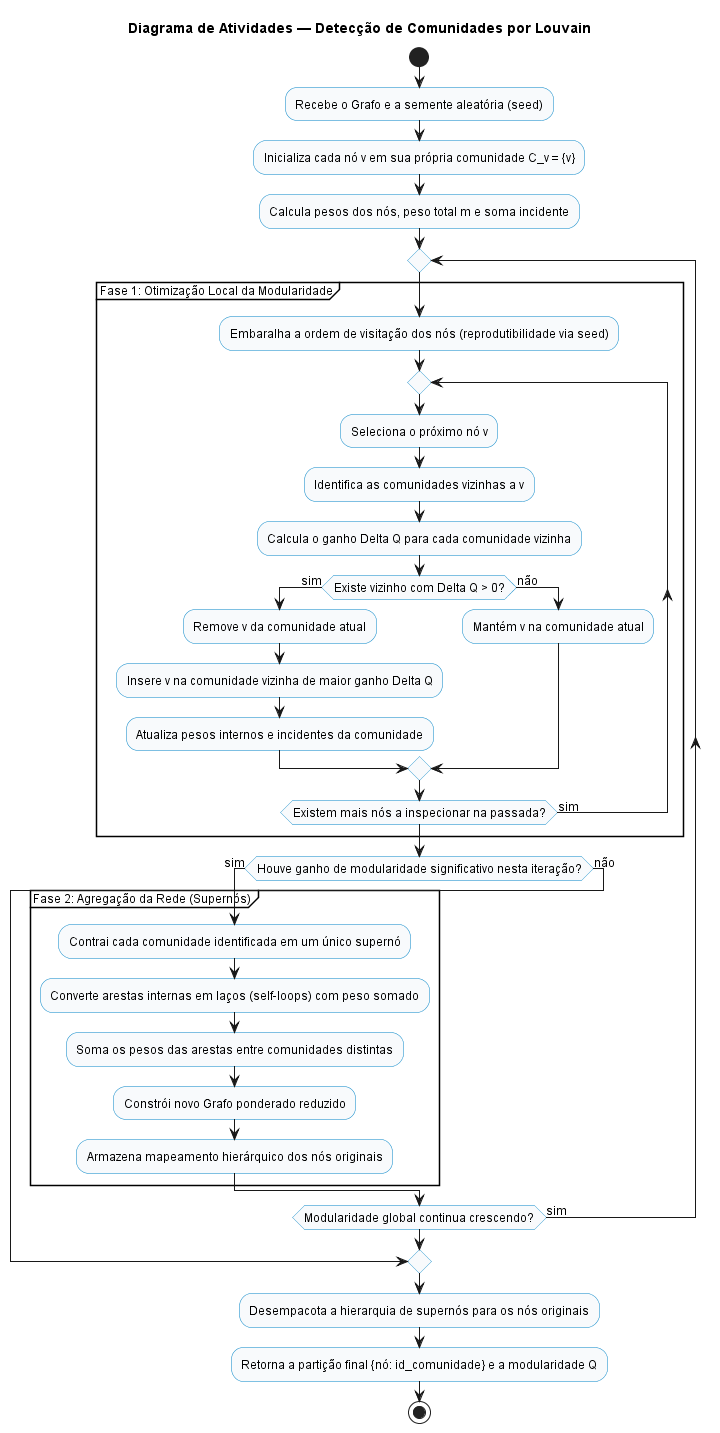
\includegraphics[width=.85\textwidth]{atividades_louvain.png}
\caption{Diagrama de atividades do algoritmo de Louvain.}
\label{fig:atividades}
\end{figure}
     % Arthur
% =====================================================================
% Plano de desenvolvimento --- Vitória (Frente 2)
% Só a Vitória edita este arquivo. A tabela de marcos foi copiada da divisão
% de tarefas; a Vitória revisa e completa com o plano dela.
% =====================================================================
\section{Plano de desenvolvimento}\label{sec:plano}

O trabalho é dividido em seis frentes de código, uma por integrante, que avançam em paralelo
a partir da classe \codigo{Grafo}. Cada função entra na \codigo{main} por \emph{pull request},
revisada por outro integrante e com os testes passando. O andamento é acompanhado num
cronograma compartilhado. A Tabela~\ref{tab:marcos} mostra os marcos.

\begin{table}[htbp]
\centering
\caption{Marcos do trabalho. A entrega final no Canvas é até 22/11/2026.}
\label{tab:marcos}
\small
\begin{tabularx}{\textwidth}{@{}l l Y@{}}
\toprule
Marco & Data & O que precisa estar pronto \\
\midrule
Base pronta (Etapa 1) & 10/11 & Classe \codigo{Grafo} e leitores na \codigo{main}; este documento \\
Algoritmos (Etapa 2) & 17/11 & Funções de cada frente na \codigo{main}, com os testes batendo com os valores de referência \\
Integração (Etapa 2) & 19/11 & Interface com as seis telas; SIR e ranking na Twitch PT; medições de desempenho \\
Entrega (Etapa 3) & 21/11 & Relatório SBC de 12 a 15 páginas, slides, vídeo e o \codigo{.zip} no Canvas \\
\bottomrule
\end{tabularx}
\end{table}

\pendente{Vitória: completar com o plano de desenvolvimento (fases, dependências entre as
frentes e riscos) e atualizar as datas, se o grupo remarcar algum marco.}
          % Vitória
% =====================================================================
% Responsabilidades de cada integrante --- Brunno
% =====================================================================
\section{Responsabilidades}\label{sec:responsabilidades}

A Tabela~\ref{tab:responsabilidades} mostra a frente de código e as partes dos documentos de
cada integrante. Os commits de cada um ficam no histórico do repositório Git do grupo.

\begin{table}[htbp]
\centering
\caption{Divisão de tarefas do grupo.}
\label{tab:responsabilidades}
\small
\begin{tabularx}{\textwidth}{@{}l Y Y@{}}
\toprule
Integrante & Frente de código & Etapa 1 \\
\midrule
Brunno & 1. Estrutura do grafo, leitores das bases e geradores sintéticos & Bases, modelagem, diagrama de classes e montagem do documento \\
Vitória & 2. Grau, caminhos (BFS, DFS, Dijkstra) e proximidade & Plano de desenvolvimento \\
Iago & 3. Centralidades (Brandes, PageRank, k-core) e desempenho & Diagrama de sequência \\
Arthur & 4. Agrupamento e comunidades (Louvain, propagação de rótulos) & Diagrama de atividades do Louvain \\
Ravi & 5. Influenciadores (SIR e comparação dos rankings) & Descrição formal do problema \\
Kaio & 6. Interface e visualização & Casos de uso e esboço das telas \\
\bottomrule
\end{tabularx}
\end{table}
 % Brunno

\bibliographystyle{sbc}
\bibliography{referencias}

\end{document}
